\documentclass{standalone}

% math and formulas
\usepackage{amsmath}
\usepackage{amsfonts}
\usepackage{amssymb}
\usepackage[amssymb]{SIunits}
\usepackage{mathtools}
\usepackage{esvect} % for vector typesetting
\usepackage{bm} % for matrix typesetting
\usepackage{xfrac}

\usepackage{environ}


% ---Notation macros---

% math
\let\oldvec\vec
% \renewcommand{\vec}[1]{\bm{\mathbf{#1}}}
\renewcommand{\vec}[1]{\bm{#1}} % \bm vs \mathbf
\newcommand{\vecf}[1]{\bm{#1}} % \bm vs \mathbf
\newcommand{\vecelem}[1]{#1}
\newcommand{\vecarrow}[1]{\vv{#1}}
\newcommand{\mat}[1]{\bm{#1}}
\newcommand{\matelem}[1]{\mathit{#1}}
\newcommand{\ten}[1]{\mathbf{#1}}
\newcommand{\tenelem}[1]{\mathrm{#1}}
\newcommand{\set}[1]{\mathbb{#1}}

\newcommand{\trans}[1]{#1^{\mathsf{T}}}
\newcommand{\ifrac}[2]{\sfrac{#1}{#2}}
\newcommand{\deriv}[2]{\frac{\text{d}#1}{\text{d}#2}}
\newcommand{\partderiv}[2]{\frac{\partial #1}{\partial #2}}
\newcommand{\ideriv}[2]{\ifrac{\text{d}#1}{\text{d}#2}}
\newcommand{\ipartderiv}[2]{\ifrac{\partial #1}{\partial #2}}

\DeclarePairedDelimiter{\norm}{\lVert}{\rVert}

% machine learning
\newcommand{\param}{\lambda}


% misc
\newcommand{\keyword}[1]{\textbf{#1}}
\newcommand{\para}{\par\medskip}
\newcommand{\ds}{\displaystyle}

\newcommand{\keycode}[1]{\texttt{#1}}
\newcommand{\code}[1]{\texttt{#1}}


\let\oldcite\cite
\renewcommand{\cite}[1]{{\color{red}(\oldcite{#1})}\\}



% --- TIKZ ---

\NewEnviron{defbox}[1]
{
  \centering

  \tikzstyle{mybox} = [draw=red, fill=blue!40!pagecolor, very thick, rectangle, rounded corners, inner sep=10pt, inner ysep=20pt]
  \tikzstyle{fancytitle} = [fill=red, text=white]
  \begin{tikzpicture}
    \node [mybox] (box) {%
      \begin{minipage}{1.0\textwidth}
        \BODY
      \end{minipage}
    };
    \node [right,inner xsep=1em,fill=red!75, text=white,outer sep=0pt,text height=2ex,text depth=.5ex] (title)
    at ([shift={(-1em,0pt)}]box.north west) {#1};
    \fill[red!50!black] (title.north east) -- +(-1em,1em) -- +(-1em,0) -- cycle;
    \fill[red!50!black] (title.south west) -- +(1em,-1em) -- +(1em,0) -- cycle;

  \end{tikzpicture}
}


\NewEnviron{infobox}[1]
{
  \centering

  \tikzstyle{mybox} = [draw=blue, fill=green!40!pagecolor, very thick, rectangle, rounded corners, inner sep=10pt, inner ysep=20pt]
  \tikzstyle{fancytitle} = [fill=blue, text=white]
  \begin{tikzpicture}
    \node [mybox] (box) {%
      \begin{minipage}{1.0\textwidth}
        \BODY
      \end{minipage}
    };
    \node [right,inner xsep=1em,fill=blue!75, text=white,outer sep=0pt,text height=2ex,text depth=.5ex] (title)
    at ([shift={(-1em,0pt)}]box.north west) {#1};
    \fill[blue!50!black] (title.north east) -- +(-1em,1em) -- +(-1em,0) -- cycle;
    \fill[blue!50!black] (title.south west) -- +(1em,-1em) -- +(1em,0) -- cycle;

  \end{tikzpicture}
}


\NewEnviron{examplebox}[1]
{
  \centering

  \tikzstyle{mybox} = [draw=green, fill=yellow!40!pagecolor, very thick, rectangle, rounded corners, inner sep=10pt, inner ysep=20pt]
  \tikzstyle{fancytitle} = [fill=green, text=white]
  \begin{tikzpicture}
    \node [mybox] (box) {%
      \begin{minipage}{1.0\textwidth}
        \BODY
      \end{minipage}
    };
    \node [right,inner xsep=1em,fill=green!75, text=white,outer sep=0pt,text height=2ex,text depth=.5ex] (title)
    at ([shift={(-1em,0pt)}]box.north west) {#1};
    \fill[green!50!black] (title.north east) -- +(-1em,1em) -- +(-1em,0) -- cycle;
    \fill[green!50!black] (title.south west) -- +(1em,-1em) -- +(1em,0) -- cycle;

  \end{tikzpicture}
}

% \newcommand{\code}{\mint[frame=lines,framesep=2mm,baselinestretch=1.2,bgcolor=lightgray,fontsize=\footnotesize,linenos]{python}}

% \newenvironment{codeblock}
% {
%   \begin{minted}[frame=lines,framesep=2mm,baselinestretch=1.2,bgcolor=lightgray,fontsize=\footnotesize,linenos]{python}
% }
% {
% \end{minted}
% }

% conditional compilation
\newif\ifcp
\cptrue % if commented out -> no compilation

% \ifcp
   %% CONDITIONAL CODE
% \fi


%%% Local Variables:
%%% mode: latex
%%% TeX-master: "../main"
%%% End:


\usepackage{xcolor}
\usepackage{tikz}
\usetikzlibrary{external,3d,matrix,chains,positioning,calc,intersections,shapes,arrows,fadings,patterns,arrows.meta,quotes}
\usepackage{tikz-3dplot}
%\tikzexternalize
\usepackage{tikzpagenodes}
\usepackage{pgfplots}
\pgfplotsset{compat=1.16}

\usepackage{graphicx}
\graphicspath{{../res/}}

\usepackage{pgf-umlsd}
\usepackage{ifthen}

\begin{document}
\colorlet{pagecolor}{white}
\colorlet{textcolor}{black}

\makeatletter
\tikzoption{canvas is plane}[]{\@setOxy#1}
\def\@setOxy O(#1,#2,#3)x(#4,#5,#6)y(#7,#8,#9)%
{\def\tikz@plane@origin{\pgfpointxyz{#1}{#2}{#3}}%
  \def\tikz@plane@x{\pgfpointxyz{#4}{#5}{#6}}%
  \def\tikz@plane@y{\pgfpointxyz{#7}{#8}{#9}}%
  \tikz@canvas@is@plane
}
\makeatother

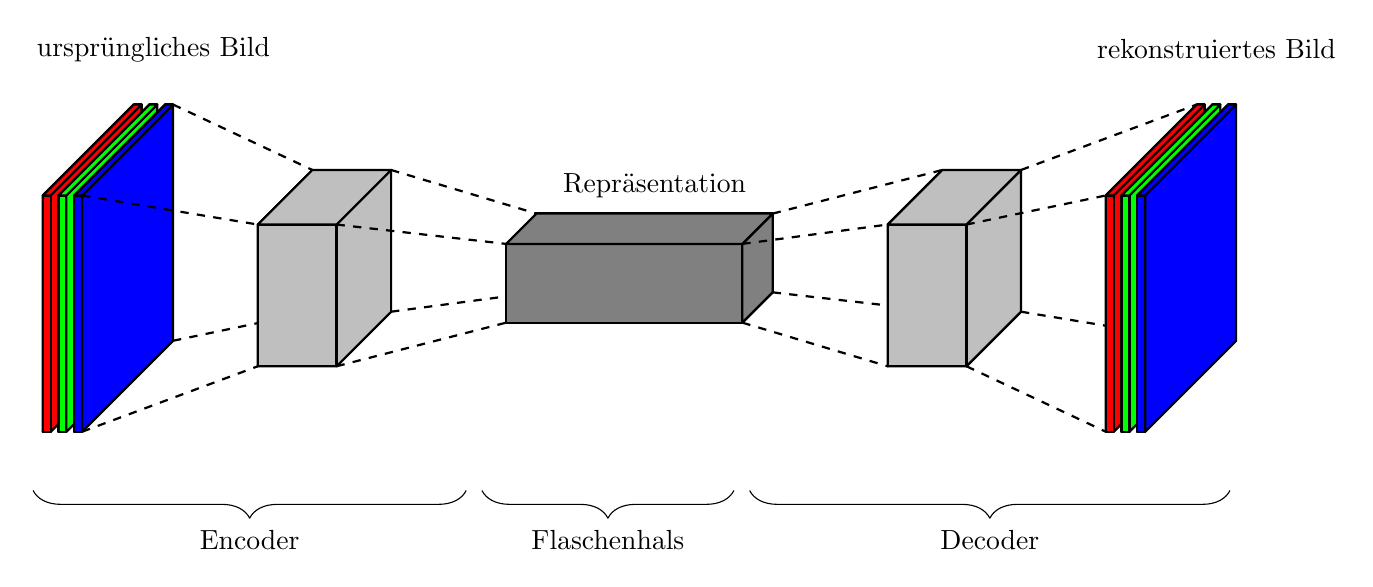
\begin{tikzpicture}[line join=round]
  \coordinate (offset) at (0,0,0);

  % #1 is size
  % #2 is depth
  % #3 is x-offset
  \newcommand{\deflayer}[4]{
    \def\s{#1/2}
    \def\d{#2}
    \def\o{#3}
    \def\c{#4}

    \coordinate (offset) at ($(offset)+(\o+\d,0,0)$);

    \coordinate (A) at ($(offset)+(-\d, -\s, \s)$);
    \coordinate (B) at ($(offset)+(0, -\s, \s)$);
    \coordinate (C) at ($(offset)+(0, \s, \s)$);
    \coordinate (D) at ($(offset)+(-\d,\s,\s)$);

    \coordinate (E) at ($(offset)+(-\d,-\s,-\s)$);
    \coordinate (F) at ($(offset)+(0, -\s,-\s)$);
    \coordinate (G) at ($(offset)+(0,\s, -\s)$);
    \coordinate (H) at ($(offset)+(-\d,\s,-\s)$);

  }

  \newcommand{\drawlayer}[0]{
    \path[draw=black,thick, fill=\c] (E) -- (F) -- (G) -- (H) -- cycle; % back
    \path[draw=black,thick, fill=\c] (E) -- (F) -- (B) -- (A) -- cycle; % bottom
    \path[draw=black,thick, fill=\c] (E) -- (A) -- (D) -- (H) -- cycle; % left
    \path[draw=black,thick, fill=\c] (B) -- (F) -- (G) -- (C) -- cycle; % right
    \path[draw=black,thick, fill=\c] (A) -- (B) -- (C) -- (D) -- cycle; % front
    \path[draw=black,thick, fill=\c] (D) -- (C) -- (G) -- (H) -- cycle; % top
  }


  \deflayer{3.0}{0.1}{0}{red}

  \coordinate(1-A) at (A);
  \coordinate(1-D) at (D);
  \coordinate(1-H) at (H);
  \coordinate(1-E) at (E);

  \drawlayer{}
  \deflayer{3.0}{0.1}{0.1}{green}
  \drawlayer{}
  \deflayer{3.0}{0.1}{0.1}{blue}
  \drawlayer{}

  \coordinate(1-B) at (B);
  \coordinate(1-C) at (C);
  \coordinate(1-F) at (F);
  \coordinate(1-G) at (G);

  \deflayer{1.8}{1}{2}{lightgray}

  \coordinate(2-A) at (A);
  \coordinate(2-B) at (B);
  \coordinate(2-C) at (C);
  \coordinate(2-D) at (D);
  \coordinate(2-E) at (E);
  \coordinate(2-F) at (F);
  \coordinate(2-G) at (G);
  \coordinate(2-H) at (H);
  \draw[thick,dashed] (1-B) -- (2-A);
  \draw[thick,dashed] (1-F) -- (2-E);
  \draw[thick,dashed] (1-C) -- (2-D);
  \draw[thick,dashed] (1-G) -- (2-H);
  \drawlayer{}

  \deflayer{1}{3}{2}{gray}

  \coordinate(3-A) at (A);
  \coordinate(3-B) at (B);
  \coordinate(3-C) at (C);
  \coordinate(3-D) at (D);
  \coordinate(3-E) at (E);
  \coordinate(3-F) at (F);
  \coordinate(3-G) at (G);
  \coordinate(3-H) at (H);
  \draw[thick,dashed] (2-B) -- (3-A);
  \draw[thick,dashed] (2-F) -- (3-E);
  \draw[thick,dashed] (2-C) -- (3-D);
  \draw[thick,dashed] (2-G) -- (3-H);
  \drawlayer{}

  \deflayer{1.8}{1}{2}{lightgray}

  \coordinate(4-A) at (A);
  \coordinate(4-B) at (B);
  \coordinate(4-C) at (C);
  \coordinate(4-D) at (D);
  \coordinate(4-E) at (E);
  \coordinate(4-F) at (F);
  \coordinate(4-G) at (G);
  \coordinate(4-H) at (H);
  \draw[thick,dashed] (3-B) -- (4-A);
  \draw[thick,dashed] (3-F) -- (4-E);
  \draw[thick,dashed] (3-C) -- (4-D);
  \draw[thick,dashed] (3-G) -- (4-H);
  \drawlayer{}

  \deflayer{3.0}{0.1}{2}{red}

  \coordinate(5-A) at (A);
  \coordinate(5-D) at (D);
  \coordinate(5-E) at (E);
  \coordinate(5-H) at (H);
  \draw[thick,dashed] (4-B) -- (5-A);
  \draw[thick,dashed] (4-F) -- (5-E);
  \draw[thick,dashed] (4-C) -- (5-D);
  \draw[thick,dashed] (4-G) -- (5-H);
  \drawlayer{}

  \deflayer{3.0}{0.1}{0.1}{green}
  \drawlayer{}
  \deflayer{3.0}{0.1}{0.1}{blue}
  \coordinate(5-B) at (B);
  \coordinate(5-C) at (C);
  \coordinate(5-F) at (F);
  \coordinate(5-G) at (G);
  \drawlayer{}

  \draw[decoration={brace,mirror,amplitude=10pt,raise=-5pt},decorate] (-0.7,-3) -- node[below=6pt] {Encoder} (4.8,-3);
  \draw[decoration={brace,mirror,amplitude=10pt,raise=-5pt},decorate] (5.0,-3) -- node[below=6pt] {Flaschenhals} (8.2,-3);
  \draw[decoration={brace,mirror,amplitude=10pt,raise=-5pt},decorate] (8.4,-3) -- node[below=6pt] {Decoder} (14.5,-3);

  \node (text_input) at ($(1-H)!0.5!(1-G)$)[yshift=20] {ursprüngliches Bild};
  \node (text_rep) at ($(3-H)!0.5!(3-G)$)[yshift=10] {Repräsentation};
  \node (text_input) at ($(5-H)!0.5!(5-G)$)[yshift=20] {rekonstruiertes Bild};

\end{tikzpicture}


%%% Local Variables:
%%% mode: latex
%%% TeX-master: "../figs"
%%% End:


\end{document}

%%% Local Variables:
%%% TeX-command-extra-options: "--shell-escape"
%%% TeX-master: "./figs"
%%% End: